\documentclass[12pt,english]{article}

%%%%%%%%%%%%%%%%%%%%%%%%%
%% SEC: PACKAGEs MAIN  %%
%%%%%%%%%%%%%%%%%%%%%%%%%
\usepackage{mathpazo}
\usepackage{eulervm}
\usepackage{amsmath}
\usepackage{amssymb}
\usepackage[utf8]{inputenc}
\usepackage[T1]{fontenc}
\usepackage{color}
% \usepackage[monochrome]{xcolor}
\usepackage{babel}
\usepackage{csquotes}
\usepackage{setspace}
\usepackage{graphicx}
\usepackage{booktabs,dcolumn}
\usepackage{array}
\usepackage{multirow}
\usepackage[font=singlespacing, skip=3pt]{caption}
\usepackage[usenames,dvipsnames,svgnames,table]{xcolor}
%\usepackage[usenames,dvipsnames,svgnames,table,monochrome]{xcolor} % test black and white color results, 2018-11-21 08:48
\usepackage{float}
\usepackage[export]{adjustbox}[2011/08/13]
\usepackage{enumitem}
% \usepackage{subfig}
%\usepackage[nolists, tablesfirst, nomarkers]{endfloat}
% \usepackage[unicode=true,pdfusetitle,
%  bookmarks=true,bookmarksnumbered=false,bookmarksopen=false,
%  breaklinks=false,pdfborder={0 0 1},backref=false,colorlinks=false]
%  {hyperref}
\usepackage[colorlinks=true, linkcolor=blue, citecolor=blue, plainpages=false, pdfpagelabels=true, urlcolor=blue]{hyperref}
\usepackage{geometry}
\usepackage{ragged2e}
\usepackage{appendix}
\usepackage{subcaption} % For subfigures

\usepackage{adjustbox}
\usepackage{siunitx}
\usepackage{indentfirst}
\newcolumntype{d}{S[input-symbols = ()]}
\usepackage{lscape}
\usepackage{longtable}
\newcommand{\source}[1]{\caption*{Source: {#1}} }
\usepackage{threeparttable} % For tables with notes
\usepackage{threeparttablex} % For extending threeparttable functionality

\usepackage{rotating}
\usepackage{pdflscape}

% Redefine the footnoterule command
\renewcommand{\footnoterule}{%
    \kern-3pt % Adjust the vertical position of the line
    \hrule width 0.2\columnwidth height 0.4pt % Width and height of the line
    \kern2.6pt % Adjust the spacing between the line and the footnotes
}

\renewcommand{\thetable}{\arabic{table}}
\renewcommand{\thefigure}{\arabic{figure}}

% *****************************************************************
% Estout LaTeX wrapper
% *****************************************************************

%%Original code developed by Jörg Weber: see
%% https://www.jwe.cc/2012/03/stata-latex-tables-estout/
%% andwho
%% https://www.jwe.cc/blog/


\let\estinput=\input % define a new input command so that we can still flatten the document

\newcommand{\estwide}[3]{
		\vspace{.75ex}{
			%\textsymbols% Note the added command here
			\begin{tabular*}
			{\textwidth}{@{\hskip\tabcolsep\extracolsep\fill}l*{#2}{#3}}
			\toprule
			\estinput{#1}
			\bottomrule
			\addlinespace[.75ex]
			\end{tabular*}
			}
		}	

\newcommand{\estauto}[3]{
		\vspace{.75ex}{
			%\textsymbols% Note the added command here
			\begin{tabular}{l*{#2}{#3}}
			\toprule
			\estinput{#1}
			\bottomrule
			\addlinespace[.75ex]
			\end{tabular}
			}
		}

% Allow line breaks with \ in specialcells
\newcommand{\specialcell}[2][c]{%
    \begin{tabular}[#1]{@{}c@{}}#2\end{tabular}
}

% \newcommand{\sym}[1]{\rlap{#1}}% Thanks David Carlisle


%%%%%%%%%%% End of wrapper %%%%%%%%%%%%%%%%%%%%%
    
%%%%%%%%%%% TiKz %%%%%%%%%%%%%%%%%%%%%
\usepackage{tikz}
\usetikzlibrary{shapes.geometric, arrows}

\tikzstyle{startstop} = [rectangle, rounded corners, minimum width=3cm, minimum height=1cm,text centered, draw=black, fill=red!30]

\tikzstyle{io} = [trapezium, trapezium left angle=70, trapezium right angle=110, minimum width=3cm, minimum height=1cm, text centered, text width =5cm, draw=black, fill=blue!30]

\tikzstyle{process} = [rectangle, minimum width=3cm, minimum height=1cm, text centered, text width =5cm, draw=black, fill=orange!30]

\tikzstyle{decision} = [diamond, minimum width=3cm, minimum height=1cm, text centered, draw=black, fill=green!30]

\tikzstyle{arrow} = [thick,->,>=stealth]

%%%%%%%%%%%%%%%%%%%%%%%%%
%% SEC: Indentation  %%
%%%%%%%%%%%%%%%%%%%%%%%%%
\geometry{
	a4paper,
	noheadfoot=true,
	left=1.0in,
	right=1.0in,
	top=1.0in,
	bottom=1.0in,
}
\setlength{\parindent}{15pt}
\makeatletter
%\doublespacing
\onehalfspacing
% \date{January 16, 2019}
\date{\today}
%\date{}

%%%%%%%%%%%%%%%%%%%%%%%%%
%% SEC: new commands  %%
%%%%%%%%%%%%%%%%%%%%%%%%%
%\exhyphenpenalty=10000\hyphenpenalty=10000
\newcommand\invisiblesection[1]{%
	\refstepcounter{section}%
	\addcontentsline{toc}{section}{\protect\numberline{\thesection}#1}%
	\sectionmark{#1}}

\newcommand{\rowgroup}[1]{\hspace{-0.5em}#1}

\newcommand*\samethanks[1][\value{footnote}]{\footnotemark[#1]}
\newcommand{\sym}[1]{\ifmmode^{#1}\else\(^{#1}\)\fi}


%%%%%%%%%%%%%%%%%%%%%%%%
%% SEC: Footer  %%
%%%%%%%%%%%%%%%%%%%%%%%%
\usepackage{calc}
\setlength{\footskip}{\paperheight
	-(1in+\voffset+\topmargin+\headheight+\headsep+\textheight)
	-0.75in}


% %%%%%%%%%%%%%%%%%%%%%%%%%%%%%% User specified LaTeX commands.
% \usepackage{setspace}
% \usepackage{parskip}
% \usepackage{float}
%
% \usepackage{graphicx}
% \usepackage{booktabs,dcolumn}
% \usepackage[font=singlespacing,skip=5pt]{caption}
%
% \usepackage[usenames,dvipsnames,svgnames,table]{xcolor}
%
% \usepackage[margin=1in]{geometry}
%
%
% \usepackage{mathpazo} % add possibly `sc` and `osf` options
% \usepackage{eulervm}
%
% \usepackage[bottom]{footmisc}
%
% %%%%%%%%%%%%%%%%%%%%%%%%%%%%%5
% %% Recent addition
% %%%%%%%%%%%%%%%%%%%%%%%%%%%%%5
\usepackage{mathtools} % for \coloneqq, 2018-08-27 10:49
\usepackage{accents} % for double dilta 2018-11-16 17:49
\newcommand{\dbtilde}[1]{\accentset{\approx}{#1}}
\usepackage[outdir=./]{epstopdf} % to include eps files, 2018-11-19 08:59
% 2018-11-21 08:51 black and white testing of eps graphs
\usepackage{xspace} % 2018-11-22 15:07 added for newcommand space problem

% 2018-12-03 11:28: color box to generate legend for equilibrium results plots
\usepackage[most]{tcolorbox}
% \definecolor{background}{HTML}{FCF9EE}
% \definecolor{background}{HTML}{FFFFFF}
\definecolor{background}{HTML}{f2f2f2}
% \definecolor{linecolor}{HTML}{581810}
\definecolor{linecolor}{HTML}{000000}
\AtBeginEnvironment{tcolorbox}{\scriptsize}

% For capitalization Needs
\usepackage{mfirstuc}

% More Math
% \usepackage{pgfmath}

% 2018-12-30 13:02
\usetikzlibrary{positioning}

% 2019-01-02 19:32, to allow for multiple footnotes together
\usepackage[multiple]{footmisc}

% 2019-01-07 11:34, to allow for calculations
\usepackage{calculator}

%
%
% \setlength{\parskip}{1mm}
%
% \setlength{\parindent}{20pt}
% \large
% \date{\today}
%
% \onehalfspace
%
% \fboxsep=2mm%padding thickness
% \fboxrule=0.5pt%border thickness
%
% %\exhyphenpenalty=10000\hyphenpenalty=10000

%%%%%%%%%%%%%%%%%%%%%%%%%%%%%%%%%%%%%%%%%%%%%%%%%%%%%%%%%%%%%%%%%%%%%%
%%% Table formatting, 2018-08-27 16:57, for equilibrium solution table
%%%%%%%%%%%%%%%%%%%%%%%%%%%%%%%%%%%%%%%%%%%%%%%%%%%%%%%%%%%%%%%%%%%%%%

\usepackage{array}
\usepackage{makecell}
\renewcommand\theadalign{bc}
\renewcommand\theadfont{\bfseries}
\renewcommand\theadgape{\Gape[4pt]}
\renewcommand\cellgape{\Gape[4pt]}

\newcolumntype{L}[1]{>{\raggedright\let\newline\\\arraybackslash\hspace{0pt}}m{#1}}
\newcolumntype{C}[1]{>{\centering\let\newline\\\arraybackslash\hspace{0pt}}m{#1}}
\newcolumntype{R}[1]{>{\raggedleft\let\newline\\\arraybackslash\hspace{0pt}}m{#1}}


%%%%%%%%%%%%%%%%%%%%%%%%%%%%%%%%%%%%%%%%%%%%%%%%%%%%%%%%%%%%%%%%%%%%%%
%%% Common Section Headings
%%%%%%%%%%%%%%%%%%%%%%%%%%%%%%%%%%%%%%%%%%%%%%%%%%%%%%%%%%%%%%%%%%%%%%

\renewcommand{\section}{\@startsection {section}{1}{\z@}%
             {-3.5ex \@plus -1ex \@minus -.2ex}%
             {2.3ex \@plus .2ex}%
             {\normalfont\Large\scshape\bfseries}}

\renewcommand{\subsection}{\@startsection{subsection}{2}{\z@}%
             {-3.25ex\@plus -1ex \@minus -.2ex}%
             {1.5ex \@plus .2ex}%
             {\normalfont\large\scshape\bfseries}}

\renewcommand{\subsubsection}{\@startsection{subsubsection}{2}{\z@}%
             {-3.25ex\@plus -1ex \@minus -.2ex}%
             {1.5ex \@plus .2ex}%
             {\normalfont\normalsize}}

%%%%%%%%%%%%%%%%%%%%%%%%%%%%%%%%%%%%%%%%%%%%%%%%%%%%%%%%%%%%%%%%%%%%%%
%%% Edit Notes
%%%%%%%%%%%%%%%%%%%%%%%%%%%%%%%%%%%%%%%%%%%%%%%%%%%%%%%%%%%%%%%%%%%%%%

\newcommand{\EDIT}[2]{\textit{#1 (\textcolor{red}{\textbf{EDIT}} #2)}}
\newcommand{\REFE}[1]{\textit{#1 (\textcolor{blue}{\textbf{R}})}}

%%%%%%%%%%%%%%%%%%%%%%%%
%% SEC: Bibliography %%
%%%%%%%%%%%%%%%%%%%%%%%%
\usepackage[authordate,
backend=biber,
doi=only,
isbn=false,
sorting=nyt,
maxcitenames=3,
minbibnames=7,
maxbibnames=7,
uniquename=false,
sortcites=true]{biblatex-chicago}

\bibliography{references.bib}

\AtEveryBibitem{\clearlist{note}\clearlist{language}\clearlist{issn}} % clears issn
\AtEveryBibitem{%
	\ifentrytype{online}{%
		\clearfield{urlyear}
		\clearfield{urlmonth}
		\clearfield{urlday}
		\clearfield{note}
		\clearlist{language}
	}{%
		\clearfield{eprint}%
% 		\clearfield{url}
		\clearfield{urlyear}
		\clearfield{urlmonth}
		\clearfield{urlday}
		\clearfield{note}
		\clearlist{language}
	}
}%


\bibliography{bib/bibliography}

\makeatother

\begin{document}

\title{The Impact of Hispanic Last Names and Identity on Labor Market Outcomes}

\author{\href{https://hussainhadah.com/}{Hussain Hadah} \thanks{Hussain Hadah: Department of Economics, Tulane University, 6823 St. Charles Ave., New Orleans, LA 70118, United States (e-mail: \href{mailto:hhadah@tulane.edu}{hhadah@tulane.edu}). I thank Professors Willa Friedman, Chinhui Juhn, Vikram Maheshri, and Yona Rubinstein for their support and advice. I also thank Aimee Chin, Steven Craig, German Cubas, Elaine Liu, Fan Wang, and the participants of the Applied Microeconomics Workshop at the University of Houston.}}


\maketitle

\begin{center}
\href{https://hhadah.github.io/hispanic-last-names/my_paper/Hadah-last-names-draft.pdf}{\textcolor{green!15!black!30!blue}{\footnotesize{\textsc{Click Here to Get the Most Updated Version}}}}
\end{center}

\begin{abstract}
\singlespacing Do people with ethnically Hispanic names face discrimination in the labor market? In this study, I analyze the causal impact of Hispanic-sounding surnames on wages, using the unique context of inter-ethnic marriages and the distinct characteristics of White and Hispanic surnames. I compare the wages of individuals with one White and one Hispanic parent, observing that those with Hispanic surnames often encounter wage disparities. The findings in this paper show a significant wage difference favoring individuals with White or native sounding surnames. Although males born to Hispanic fathers and White mothers earn 5 percentage points less than those born to White fathers and Hispanic mothers, this gap can be completely attributed to differences in education levels. However, this should not be interpreted as an absence of discrimination; rather, it potentially reflects discrimination in access to education. Additionally, I explore the impact of self-identifying as Hispanic on earnings. Men with a Spanish-sounding last name who identify as Hispanic earn significantly less than those who do not, but again, this gap can be largely explained by educational disparities. This suggests that discrimination may extend beyond the labor market, influencing educational opportunities and outcomes too.


\end{abstract}

\noindent\textbf{Keywords}: Economics of Minorities, Race, and Immigrants; Discrimination and Prejudice

\noindent\textbf{JEL Classification}: J71; J64; J15

\vfill
\pagebreak{}

\section{Introduction}\label{sec:intro}

A large literature documents substantial earnings gaps across race and ethnicity \autocite{bayer2018divergent, charles2008prejudice, card1992school, fryer2004causes, rubinstein2014pride, bertrand2004emily, juhn1991accounting}. Hispanics constitute a large and growing portion of the population in the United States. As the number of Hispanics increases, determining whether ethnic discrimination affects their labor market outcomes becomes increasingly crucial \autocite{chettyUnitedStatesStill2014, chettyEffectsExposureBetter2016,chettyFadingAmericanDream2017,abramitzkyImmigrantsAssimilateMore2020a, abramitzkyNationImmigrantsAssimilation2014,abramitzkyCulturalAssimilationAge2016,chettyWhereLandOpportunity2014}. Thus, it is important to understand whether a person's ethnicity affects their labor market outcomes. Assimilation and mobility are crucial because they reflect how well Hispanics can integrate into society and move up the socioeconomic ladder.

In this paper, I answer the following questions. Does having a Hispanic last name affect labor market outcomes? What is the effect of identifying as Hispanic on earnings? Moreover, I aim to show that comparing Hispanic Whites to non-Hispanic Whites might create an artificially higher earnings gap since the two groups differ on many observable characteristics.\footnote{By identifying as Hispanic, I refer to individuals who self-report their ethnicity as Hispanic on surveys or other data collection instruments.} \footnote{Observable characteristics refer to factors that can be measured and quantified, such as education level, work experience, and immigration status.} Others have attempted to compare how native-born White Hispanics fare to non-Hispanic Whites and foreign-born Hispanics. In \textcite{antman2020ethnic,antmanEthnicAttritionObserved2016,antmanEthnicAttritionObserved2016a,antmanEthnicAttritionAssimilation2020}, the authors compare the health and educational outcomes of Hispanic Whites to non-Hispanic Whites and native-born Hispanics to foreign-born Hispanics. They find gaps in education and health between Hispanics and Whites. They also find that native-born Hispanics are more likely than their foreign-born counterparts to report poor health. \textcite{davilaChangesRelativeEarnings2008} documents many gaps in labor market outcomes between Hispanics and Whites. They attribute a big part of this gap to differences in education, experience, immigration status, and regional differences. 

The US population is growing in diversity. The proportion of non-Whites has increased by more than 10 percentage points from 13 percent in 1995 to 23 percent in 2019. The number of Hispanics has grown by 9 percentage points from 9 percent in 1995 to 16 percent in 2019.\footnote{The portion of non-Whites and Hispanics is calculated using the Current Population Survey (CPS).} Native-born White Hispanic men earn 21\% less than White men, although a substantial portion of the earnings gap is due to educational differences between Hispanics and Whites \autocite{duncan2006hispanics, duncan2018identifying, duncan2018socioeconomic}. Some of the earnings differences may also be due to discrimination which will have negative consequences. For example, discrimination against Hispanics can lead to reduced job opportunities, lower wages, and hinder assimilation. In this paper, I examine the role of having a Hispanic last name and identifying as Hispanic on labor market outcomes. 

Identifying discrimination is difficult because of factors that affect labor market outcomes that are unobservable to economists---such as unobserved skills and separating it from prejudice and stereotypes. One strategy used by researchers is audit or resume studies. \textcite{bertrand2004emily} conducted an audit study where identical resumes were sent to employers with White and Black-sounding names. This approach, however, has its drawbacks. Audit studies only observe callbacks, not wages. 

This study utilizes a method developed by \textcite{rubinstein2014pride}. I compare children from inter-ethnic marriages. More precisely, I compare children of Hispanic fathers and White mothers (henceforth HW) to children of White fathers and Hispanic mothers (henceforth  WH). This approach stems from the fact that there is a strong selection among many characteristics, and thus, marriages are not random. Couples match on several observable characteristics like income, schooling, socio-economic background, etc. \autocite{averettBetterWorseRelationship2008, averettEconomicRealityBeauty1996, beckerTheoryMarriagePart1973, beckerTheoryMarriagePart1974, beckerTreatiseFamily1993, browningCollectiveUnitaryModels2006, chiapporiFatterAttractionAnthropometric2012}. Children of HW and WH marriages have more similar observable characteristics than children of endogamous/homogamous marriages--- i.e., White fathers-White mothers and Hispanic fathers-Hispanic mothers. Moreover, children from a Hispanic father and White mother household will have a Hispanic last name from their fathers, enabling the investigation of how ethnic signals, such as having a Hispanic last name, affect annual log earnings.

The main identifying assumption of my empirical strategy depends on the assumption that people born to Hispanic fathers and White mothers are similar to their White fathers Hispanic mothers peer in all observable aspects and characteristics that are important in the labor market. Consequently, the only difference between the two groups is the variation in which group is more likely to have a Hispanic sounding last name. Children from mixed ethnic backgrounds may appear physically similar to those from single ethnicity backgrounds, but the influence of family dynamics and upbringing, crucial in developing skills and personal characteristics, varies with the pattern of mixed ethnic marriages. Particularly in a society where Hispanic ancestry is perceived negatively, it raises the question of what kind of White women would choose Hispanic men. Furthermore, even if such unions were formed randomly, children from White-Hispanic homes might benefit from more favorable family conditions than those from Hispanic-White homes, considering Whites generally have stronger socio-economic backgrounds than Hispanics. These factors introduce doubts regarding whether children from Hispanic-White families receive comparable familial support and influences, either genetically or environmentally, as those from White-Hispanic families.

Previous studies have also used names as a proxy for race and ethnicity \autocite{fryer2004causes, rubinstein2014pride, bertrand2004emily}. \textcite{fryer2004causes} point out that names can be a predictor of a person's race. Specifically, they provide a rising pattern among Blacks having different names than Whites. They did, however, find that having a Black name, after controlling for the home environment at birth, does not affect their labor market outcomes. \textcite{rubinstein2014pride} compared the children of mixed marriages between Sephardic and Ashkenazi Jews in Israel.\footnote{Ashkenazi and Sephardic are two distinct Jewish ethnic groups.} They found that workers with Sephardic last names earn substantially less than those with Ashkenazi last names. \textcite{bertrand2004emily} conducted an audit study by sending employers identical resumes that differ in the ethnic and racial signal of a name (Black sounding name versus a White sounding one). They found that resumes with Black-sounding names received substantially fewer callbacks than their White counterparts. 

Using the Current Population Survey (CPS) from 1994 to 2019 and the 1960 to 2000 US censuses, I estimate the effect of having a Hispanic last name on labor market outcomes. In other words, I approximate the variation in labor market perception of ethnic signals, in this case having a Hispanic last name, on annual log earnings. I also study the effect of identifying as Hispanic on labor market outcomes. 

I find that while men born to Hispanic father-White mothers earn less than men born to White father-Hispanic mothers, this gap is entirely explained by educational differences. I find that inter-ethnic children with Hispanic sounding last name earn 5 percentage points less than those without a Hispanic last name. The gap becomes statistically insignificant after controlling for education. Thus, I do not find a significant effect of having a Hispanic last name. Finally, I find that men identifying as Hispanic earn significantly less than those who do not, even when I control for ancestry and education.


The rest of the paper is organized as follows. Section \ref{sec:data} provides an overview of the data and summary statistics of the sample. Section \ref{sec:emp_model} introduces the empirical framework. I report the results in section \ref{sec:results}. Finally, I offer a brief conclusion in section \ref{sec:con1}.

\section{Data}\label{sec:data}

I use two datasets:  the Integrated Public Use Microdata Series (IPUMS) Current Population Survey (CPS) Annual Social and Economic (ASEC) \autocite{cps2019} and the 1960 to 2000 US censuses \autocite{acs2019}. 

I use the CPS data set to study the effect of having a Hispanic last name on a person's labor market outcomes. I take advantage of the fact that the CPS asks parents' place of birth, ethnicity, and race. The data spans the period between 1994--- the earliest sample to ask about a parent's place of birth--- to 2019. Moreover, since the CPS does not provide data on parents' characteristics, essential to determine the family background, I use the census to construct synthetic parents. The census offers a larger sample of potential parents. Similar to the CPS, the 1960 to 2000 censuses ask about the person's place of birth and the individual's race and ethnicity. I employ this information to construct "synthetic parents" using a method developed by \textcite{rubinstein2014pride}. I construct the synthetic parents by linking husbands and wives in the census data to each other. I assume that parents have children between the ages of 25 and 40. I then link these synthetic parents using the birth year of child, and parents' places of birth to the year of birth of the "children" and the parents' places of birth in the CPS sample.

\subsection{Children of the four parental types}

I use the CPS for my primary analysis of the effect of having a Hispanic last name on earnings. I restrict my sample to people that racially identified as White, United States-born citizens aged 25 to 40 and born between 1960 to 2000. Taking advantage of data on parents' place of birth, I divide the sample into four groups depending on their parent's ethnicity. Mothers or fathers are Hispanic if they were born in a Spanish-speaking country and Puerto Rico, and White if they were born in the United States.\footnote{The list of Spanish Speaking countries include: Argentina, Bolivia, Chile, Colombia, Costa Rica, Cuba, Dominican Republic, Ecuador, El Salvador, Guatemala, Equatorial Guinea, Honduras, Mexico, Nicaragua, Panama, Paraguay, Peru, Spain, Uruguay, Venezuela.} Therefore, an observation can be the product of four types of parents: 
\begin{enumerate}
\item White father and White mother (hereafter WW) 
\item White father and Hispanic mother (hereafter WH)
\item Hispanic father and White mother (hereafter HW)
\item Hispanic father and Hispanic mother (hereafter HH).
\end{enumerate}

The distribution of the four types of children is presented Table \ref{tab:mat1}. The majority of the sample (96\%) is WW children. The second biggest group is HH, which constitutes 3\% of the sample. Inter-ethnic children, WH and HW, make up 1.35\% of the sample with 90,325 observations. Even though WH and HW are only 1.35\% of the sample, I have plenty of observations to carry out an analysis. The summary statistics for the children of the four types of marriages are presented in Table \ref{tab:c&p1}. Children of WW marriages (column 1) do better on every measure while children of HH parents (column 4) do worse than other children on every measure. Children of WH (column 2) and HW (column 3) marriages fall in between WW and HH children. Moreover, the summary statistics for those that also identify as Hispanic is reported in in Table \ref{tab:c&p2}.

 
\subsection{Synthetic parents}

Using the 1960 to 2000 censuses, I constructed a data set of synthetic parents. The sample includes married White men and women. Even though the census asks a person whether they are Hispanic or not, I took advantage of the questions on place of birth to create a proxy for ethnicity. I consider a Hispanic person as White and born in a Spanish-speaking country. Consequently, Whites in the sample are people who are White and native-born. Using the information provided in the census, I can link husbands and wives with each other. I assume that parents have children between the ages of 25 and 40. Therefore, my sample consists of married White men and women with children that were born in the 1920 to 1975 cohorts\footnote{The construction of "synthetic parents" follows the method used by \textcite{rubinstein2014pride}.}.

I show the distribution of the four types of couples in Table \ref{tab:mat2}. White husbands and White wives (WW) make up the majority of couples in the sample, 96\% (5,141,737 couples). Hispanic husbands and wives (HH) are the second largest group making up 2\% (119,749 couples) of all couples. White husbands and Hispanic wives (WH) couples are less 1\% (33,097 couples) of the sample and Hispanic husbands and White wives (HW) are also 1\% (37,847 couples). I present the summary statistics of the parents in Table \ref{tab:synth}.

\section{Empirical Strategy}\label{sec:emp_model}

In this section, I present two empirical strategies. The first empirical strategy estimates the effect of having a Hispanic last name on annual log earnings. The second empirical strategy estimates the effect of identifying as Hispanic on log annual earnings.

The difference in means between Hispanics and non-Hispanic Whites could result from discrimination. It can also be caused by differences in innate abilities, skills, and parental investments. While controlling for observable skill measures, I compare children of inter-ethnic marriages, HW and WH. WH and HW children are more similar in characteristics but provide employers, and the labor market, with different signals.\footnote{WH and HW children are both half White, half Hispanic.} WH children will have a non-Hispanic last name, while HW children will have a Hispanic last name. This is a method developed by \textcite{rubinstein2014pride}.

\subsection{Estimating the effect of having a Hispanic last name}

In this section I restrict the sample to WH and HW groups. Let $Y_{ist}$ be the annual log earnings of person $i$ in state $s$ at time $t$. $HW_{ist}$ is an indicator variables for the type of parents of person $i$ has. $X_{ist}$ is a vector of controls that includes age and numbers of hours worked, $\gamma_{t}$ are year fixed effects, $\lambda_{s}$ are state fixed effects, and $\phi_{ist}$ represents the error term. The equation for this strategy is written as follows:
\begin{equation} \label{eq:1a}
Y_{ist} = \beta_{1} HW_{ist} + X_{ist} \pi + \gamma_{t} + \lambda_s + \phi_{ist}
\end{equation}

$\beta_{1}$ is the coefficient of interest in this specification. $\beta_{1}$ represents the earnings gaps between children of inter-ethnic marriages who have a Spanish-sounding last name versus a White last name.

\subsection{Estimating the effect of identifying as Hispanic}

In this section, I will present an estimation strategy that would allow me to capture the effect of identifying as a Hispanic. 

\begin{equation} \label{eq:iden}
Y_{ist} = \beta_{1} HW_{ist} + \beta_{2} Hispanic_i + \beta_{3} HW_{ist} \cdot Hispanic_i + X_{ist} \pi + \gamma_{t} + \lambda_s + \phi_{ist}
\end{equation}

The coefficients of interest from equation \ref{eq:iden} are $\beta_{1}$, $\beta_{2}$ and $\beta_{3}$. The coefficients $\beta_{1}$ and $\beta_{3}$ capture the effects of Spanish-sounding last names for $HW_{ist}$ that identify as Hispanic \textit{versus} those who do not.

\subsection{Threats to Identification}

The central assumption underpinning my estimation strategy is based on the hypothesis that individuals born to a Hispanic father and White mother exhibit comparable characteristics to their peers of White-Hispanic descent, especially in areas vital to the labor market. This assumption includes similarities in educational background, skill sets, and work experiences that are significant determinants in employment opportunities, salary levels, and career advancement. 

Two primary reasons underscore that this assumption. First, there is a significant selection in the marriage market. Since belonging to the Hispanic out-group comes with a negative penalty in society, one might wonder who are the White women that would be willing to give their kids a Hispanic last-name that would potentially negatively influence their futures. Second, fathers and mothers influence human capital accumulation differently \autocite{kimball2009risk,magruder2010intergenerational}. If marriage was random, then WH households might be a better environment for children that HA. Using the CPS and the US Census, I will evaluate these empirical concerns. 

The previous two threats to identification could be addressed by the selection of partners among inter-ethnic couples. The average White person exhibits better observable characteristics than the Average Hispanic. Consequently, if marriages were random, the White husband in an WH marriage would have better traits than wife, and the White wife in the HW marriage would have the stronger traits. The random matching coupled with the fact that parents are not perfect substitutes in the inter-generational transmission of human capital would render the identification invalid since the parental background will affect labor market outcomes. 

Marriages, however, are not random. There is large body of empirical and theoretical work that indicates that marriages exhibits strong selection, or what is referred to as assortative matching, on traits \autocite{averettBetterWorseRelationship2008, averettEconomicRealityBeauty1996, beckerTheoryMarriagePart1973, beckerTheoryMarriagePart1974, beckerTreatiseFamily1993, browningCollectiveUnitaryModels2006, chiapporiFatterAttractionAnthropometric2012}. Also, \textcite{duncanIntermarriageIntergenerationalTransmission2011} shows a similar pattern of assortative matching among Mexicans in the United States. These papers suggest that inter-ethnic WH and HW marriages will, on average, consist of partners sharing similar characteristics. Consequently, the literature would predict that both WH and HW parents will be similar in all aspects that are relevant to a child's labor market outcomes. I will go over the empirical evidence from the data to show that this is actually the case.

Another threat to identification could arise from measurement error in using the place of birth of parents in the CPS data as a proxy for a parent's ethnicity and last name. The CPS only asks about the place of birth of parents and not their ethnic or racial identity. Therefore, it is possible that a native-born father could be a second-generation or later immigrant from a Spanish-speaking country. However, this scenario is highly improbable. Most Hispanics from 1960 to 2000 were first-generation immigrants, and the number of second-generation or later was very small. This is supported by data from the 1960 to 2000 censuses (see Table \ref{tab:mat3}). Only 3\% of native-born Americans identified as Hispanic, indicating the small number of second-generation or later Hispanic immigrants in the sample. Therefore, the probability that an inter-ethnic child with a native-born father that is also a second generation+ Hispanic immigrant is very small.


\section{From the Data: The Differences Between HW and WH Couples}\label{sec:hw-wh-couples-data}

In this section, I explore the empirical data to affirm the validity of my empirical strategy, as presented in Table \ref{tab:synth}, which details the educational and economic profiles of parents from four different ethnic groupings—White White (WW), White Hispanic (WH), Hispanic White (HW), and Hispanic Hispanic (HH). This table meticulously lays out the average outcomes and discrepancies for each group, highlighting the impact of inter-ethnic marriages on children's prospects. These results show that there is selection in marriage, and that the differences between children born to Hispanic fathers and White mother (HW) and children born to White fathers and Hispanic mother (WH) are less severe that those between the other two groups. Consequently, comparing WH and HW children to each other to analyze discrimination against Hispanics in the labor market.

Using the ``synthetic'' parents sample that I constructed using the Census data, I examine the family background of the different type of children. WW couples have higher education, 12.58 years for husbands and 12.36 for wives. As a household, WW couples have 24.95 years of schooling. Husbands in HH marriages have 8.64 years of education, while women have 8.49 years of schooling. As a household, HH couples have 17.13 years of education. As predicted, the inter-ethnic couples exhibit matching in which partners marry people similar to them. WH husbands have 11.82 years of education, while wives have an average of 10.71 years. WH household attained a total of 22.68 years of schooling in total. HW husbands have 10.33 years of education, while wives have an average of 11.01 years. HW household attained a total of 21.50 years of schooling in total. Both Hispanic men and women in inter-ethnic couples marry white spouses that are, on average, more educated the the average HH couple. More importantly for human capital accumulation, the mother in the HW marriages---the children that have a Spanish sounding last-name---are more educated than their WH peers. Since mothers could be more important in the a child's human capital accumulation and education, this would suggest that a child with a Hispanic last-name should complete more years of education. 

The data reveals that WW couples have the highest total household education, amounting to 24.95 years, significantly surpassing the 17.69 years of HH couples. This stark contrast underlines the substantial educational divide between these groups. Inter-ethnic couples, WH and HW, display intermediate educational achievements, with WH households totaling 22.68 years of education and HW households slightly behind at 21.50 years. Notably, HW husbands are less educated (10.33 years) compared to WH husbands (11.82 years), yet HW wives surpass their WH counterparts with 11.01 years of education, suggesting a balance in educational attainment within these marriages. This factor is particularly pertinent for children with Hispanic last names who might derive greater benefits from their mother's higher education.

In terms of labor market performance, WW households boast the highest log total family income at 10.75, while HH households fall at the lower end with 10.42. Among inter-ethnic couples, WH households have a slightly higher total income of 10.65 compared to HW households at 10.60. Notably, the difference in husbands' log hourly earnings between HW and WH is marginal, indicating HW men earn 4\% less than their WH counterparts. Furthermore, HW women actually surpass WH women in earnings, with HW wives earning 1.75 and WH wives earning 1.73 in log hourly earnings, respectively. This reversal in the typical earning pattern not only speaks to the closing economic disparities between these groups but also implies potentially greater economic contributions from HW women to their families, which could be advantageous for children and to the developments of traits that are important in the labor market.

The table also sheds light on fertility trends, noting that WW couples have less children than HH couples, reflecting broader socio-economic and cultural patterns. The difference in fertility between HW and WH couples is positive but significantly lower than the difference in fertility between HH and WW couples.

The evidence presented in this section supports a robust empirical strategy, revealing significant selection in marriage and distinctive educational and income patterns among different types of families. Inter-ethnic couples exhibit comparable levels of education and earnings. This suggests that the children of HW families are likely positioned for better educational outcomes, critical in understanding discrimination in the labor market. Notably, the disparities between HW and WH families are considerably less pronounced than those between other groups, emphasizing the importance of comparing these children directly. Such comparisons shed light on the nuanced dynamics of ethnicity, education, and economic outcomes in inter-ethnic marriages. \footnote{I present in Tables \ref{tab:synthmex} and \ref{tab:syntnonmex} the summary statistics which detail the educational and economic profiles of parents from four different ethnic groupings—White White (WW), White Hispanic (WH), Hispanic White (HW), and Hispanic Hispanic (HH) on sub-samples of Hispanics of Mexican and non-Mexican ancestries. I find similar results that describe a selection into inter-ethnic marriages among the two groups.} 

Despite higher levels of education and income among Hispanic White (HW) mothers compared to White Hispanic (WH) mothers, suggesting an expectation of greater educational attainment for HW children, data reveals a discrepancy. Specifically, HW children complete, on average, 0.4 fewer years of education compared to their WH peers (refer to Table \ref{tab:c&p1}). This gap may suggest potential discrimination or barriers in educational access for HW children.

\section{Results}\label{sec:results}

In this section, I present the results from estimating the two specifications presented in equations \ref{eq:1a} and \ref{eq:iden}. I estimate the mean wages of White, U.S.-born, Hispanic men aged 25-40 who are employed full-time and full-year (FTFY) as waged and salaried workers. The results are shown in Tables \ref{tab:lastnamereg} and \ref{tab:identreg}.

I find that an inter-ethnic person with a Spanish-sounding last names earns less than an inter-ethnic who has a White last name. A person with a Spanish-sounding last name earns 5 percentage points less than a person with a White last name. In other words, by comparing inter-ethnic children, a person with a Hispanic last name earns 5 percentage points less than someone with a White last name. However, more than half of the earnings gaps could be explained by educational differences. When I control for education, the last name effect decreases to a statistically insignificant 1 percentage points earnings gap. I also find a significant earnings gap between those that identify as Hispanic. 

\subsection{The Effect of Having a Hispanic Last Name and Hispanic Identity on Labor Market Outcomes}

I provide the results to the estimation of equation \ref{eq:1a} in Table \ref{tab:lastnamereg}. I estimate the mean wages of White, U.S.-born, Hispanic men aged 25-40 who are employed full-time and full-year (FTFY) as waged and salaried workers. I also restrict the sample to children of HW and WH (omitted) parents. Column one in Table \ref{tab:lastnamereg} is the average crude earnings gap in log annual earnings between HW workers and their WH peers. In the next 4 columns, I introduce the results with controls for hours worked, state FE, year FE, age FE, Education FE, and parental background. 

Overall, the crude gap between HW and WH workers is equal to 5 percentage points (Table \ref{tab:lastnamereg} column 1). An inter-ethnic with a Hispanic last name earns 5 percentage points less than an inter-ethnic with a White last name. Even after controlling for hours worked, and including state, year, and age FEs in the estimation, the gap stays at 5 percentage points. This gap, however, could be entirely explained by educational differences. An inter-ethnic with a Hispanic last name earns 1 percentage points less than an inter-ethnic with a White last name, but the result is statistically insignificant. 

Since Hispanics are a very heterogeneous group, I conduct a heterogeneity analysis on different samples of Hispanics. To increase the sample size of my analysis I estimate equation \ref{eq:1a} using weekly earnings as a dependent variable. Weekly earnings are available in all of the monthly CPS surveys and not just the March Supplement. I present the results to these estimations in tables \ref{tab:lastnamereg-weekearm}-\ref{tab:lastnamereg-weekearm-cub}. 

First, in Table \ref{tab:lastnamereg-weekearm}, I present the results to the estimation of equation \ref{eq:1a} using weekly earnings as a dependent variable on the full sample. Similar to the analysis before, I find that a person with a Hispanic last name earns 4 p.p. less that a person without a Hispanic last name. This gap could be explained by Educational differences. Second, in Table \ref{tab:lastnamereg-weekearm-mex}, I present the results to the estimation of equation \ref{eq:1a} using weekly earnings as a dependent variable on a sample of Mexican Hispanics. I find that a Mexican with a Hispanic sounding last name earns 3 p.p. less than a Mexican with a native sounding last name. The gap becomes an imprecise zero after controlling for education and parental background. Third, in Table \ref{tab:lastnamereg-weekearm-nonmex}, I present the results to the estimation of equation \ref{eq:1a} using weekly earnings as a dependent variable on a sample of non-Mexican Hispanics. The gap between non-Mexicans with Hispanic sounding last names and those with native sounding last names was similarly explained by educational differences. I find that a non-Mexican with a Hispanic sounding last name earns 3 p.p. less than a Mexican with a native sounding last name. The gap becomes an imprecise zero after controlling for education and parental background. Finally, in Table \ref{tab:lastnamereg-weekearm-cub}, I present the results to the estimation of equation \ref{eq:1a} using weekly earnings as a dependent variable on a sample of Cubans. I find that a Cuban with Hispanic sounding last name earns 4 p.p. less than a Cuban with a native sounding last name but the gap was statistically insignificant.

I provide the results to the estimation of equation \ref{eq:iden} in Table \ref{tab:identreg}. The sample in this analysis includes full-time, full-year, and wage and salary men, and I control for hours worked and age and include year fixed effects (FE). I also restrict the sample to children of HW and WH parents. The omitted group is children of WH parents that do not identify as Hispanic. Column one in Table \ref{tab:identreg} is the results without controlling for education. An inter-ethnic $HW_{ist}$ that identifies as Hispanic \textit{versus} $HW_{ist}$ who do not---i.e. $HW_{ist} + HW_{ist} \cdot Hispanic_i$---earns 6 percentage points less than an inter-ethnic that does not, but the result could be entirely explained by educational differences.

\section{Conclusion}\label{sec:con1}

As the Hispanic population grows in the United States, studying discrimination against this group becomes increasingly important. In this paper, I examine discrimination against Hispanics in the labor market. More specifically, I examine the impact of Hispanic last names and Hispanic identification on annual log earnings. 

I compare the children of inter-ethnic marriages to study the labor market impact of having a Hispanic last name. When I compare the earnings of HW and WH children, which captures the effect of having a Hispanic last name, HW children earn  6 percentage points less than WH children. Thus, by comparing inter-ethnic children, a person with a Hispanic last name makes 5 percentage points less than someone with a White last name. When I control for education, the last name effect decreases to a statistically insignificant 2 percentage points earnings gap. Moreover, I estimate the effect of identifying as Hispanic and having a Hispanic last name. I find that an inter-ethnic child with a Hispanic last name and identifies as Hispanic earns 5 percentage points less that an inter-ethnic child with native sounding last name and identifies as Hispanic. 

While the earnings gap between children of inter-ethnic parents with and without a Hispanic last name disappears when controlling for education, it does not necessarily indicate the absence of discrimination. Education itself can be influenced by bias, potentially resulting in divergent outcomes. This is especially the case when parental characteristics indicate that people with a Hispanic-sounding last-names should in theory complete more years of education---since mothers of inter-ethnic children with a Hispanic last-names have more years of education and earn more. Consequently, further research is needed to comprehensively understand the earnings gaps between Hispanics and Whites.


\pagebreak
\begingroup
\setstretch{1.0}
%\setstretch{1.1}
\setlength\bibitemsep{0pt}
\printbibliography
\endgroup
\pagebreak

\begin{appendices}
% \section{Figures}\label{appendix:figs}

% \begin{center}
% \begin{figure}[H]
% \caption{Histogram Before Targetting}
% \includegraphics[width=\textwidth]{img/hist_dep_original.jpg} 
% \label{fig:hist}
% \end{figure}
% \end{center}

% \pagebreak

% \begin{center}
% \begin{figure}[h!]
% \caption{Distribution of the four types of children.}
% 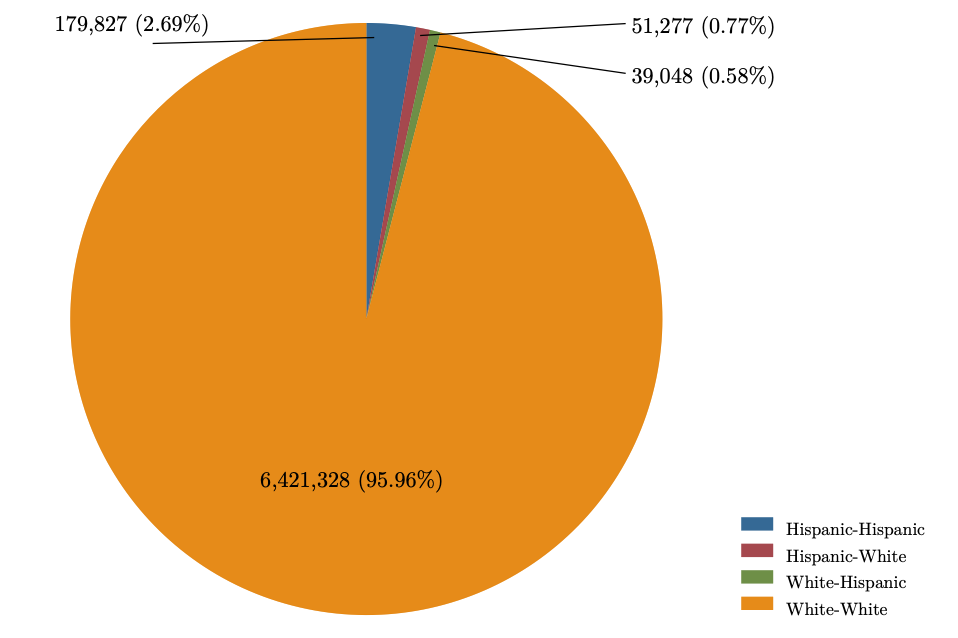
\includegraphics[width=\textwidth]{PirChart2.png} 
% \label{fig:dist}
% \end{figure}
% \end{center}

% \newpage


\section{Tables}\label{appendix:tabs}

\begin{table}[t]
\tablefont
\caption{Number of Children by Parental Type \label{tab:mat1}}
%\resizebox{\linewidth}{!}{
\begin{threeparttable}
\begin{tabular}[t]{>{}lcccc}
\toprule
\multicolumn{1}{c}{ } & \multicolumn{4}{c}{Perental Type} \\
\cmidrule(l{3pt}r{3pt}){2-5}
  & \specialcell{White Father \\ White Mother} & \specialcell{White Father \\ Hispanic Mother} & \specialcell{Hispanic Father \\ White Mother} & \specialcell{Hispanic Father \\ Hispanic Mother}\\
\midrule
\textbf{\specialcell{Observations\\Share}} & \specialcell{6,421,328\\0.96} & \specialcell{39,048\\0.01} & \specialcell{51,277\\0.01} & \specialcell{179,827\\0.03}\\
\bottomrule
\end{tabular}
\begin{tablenotes}
\item[1] Source: Current Population Surveys (CPS) 1994-2019
\item[2] The sample includes Whites, who are married, and are between the ages 25 and 40. Ethnicity of a person's parents are identified by the parent's place of birth. A parent is Hispanic if she/he was born in a Spanish-speaking country. A parent is White if she/he was born in the United States.
\end{tablenotes}
\end{threeparttable}
%}
\end{table}



\newpage


\begin{landscape}
\begin{ThreePartTable}
\begin{TableNotes}
\item[1] Source: The 1960-2000 Census for synthetic parents, and 1994-2019 Current Population Surveys (CPS) for children's outcomes
\item[2] The data is restricted to native-born United States citizens who are also White and between the ages of 25 and 40. I identify the ethnicity of a person's parents through the parent's place of birth. A parent is Hispanic if they were born in a Spanish-speaking country. A parent is White if they were born in the United States.
\end{TableNotes}
\begin{longtable}[t]{>{\raggedright\arraybackslash}p{5cm}cccccc}
\caption{Summary statistics of children's outcomes using parent's place of birth \label{tab:c&p1}}\\
\toprule
\multicolumn{1}{c}{ } & \multicolumn{4}{c}{Father's and Mother's Ethnicities} & \multicolumn{2}{c}{Differences} \\
\cmidrule(l{3pt}r{3pt}){2-5} \cmidrule(l{3pt}r{3pt}){6-7}
Variables & \specialcell{White \\ White \\ (WW) \\ (1)} & \specialcell{White \\ Hispanic \\ (WH) \\ (2)} & \specialcell{Hispanic \\ White \\ (HW) \\ (3)} & \specialcell{Hispanic \\ Hispanic \\ (HH) \\ (4)} & \specialcell{HH - WW \\ (5)} & \specialcell{HW - WH \\ (6)}\\
\midrule
\endfirsthead
\caption[]{Summary statistics of children's outcomes using parent's place of birth  \textit{(continued)}}\\
\toprule
Variables & \specialcell{White \\ White \\ (WW) \\ (1)} & \specialcell{White \\ Hispanic \\ (WH) \\ (2)} & \specialcell{Hispanic \\ White \\ (HW) \\ (3)} & \specialcell{Hispanic \\ Hispanic \\ (HH) \\ (4)} & \specialcell{HH - WW \\ (5)} & \specialcell{HW - WH \\ (6)}\\
\midrule
\endhead
\midrule
\multicolumn{7}{r@{}}{\textit{(Continued on Next Page...)}}\
\endfoot
\bottomrule
\insertTableNotes
\endlastfoot
\textbf{Panel A: Children's Education} & \textbf{} & \textbf{} & \textbf{} & \textbf{} & \textbf{} & \textbf{}\\
\hspace{1em}Men’s education (Total Years) & \specialcell{13.82\\(2.42)} & \specialcell{13.58\\(2.40)} & \specialcell{13.22\\(2.34)} & \specialcell{12.90\\(2.31)} & \specialcell{-0.92***\\(0.01)} & \specialcell{-0.36**\\(0.02)}\\
\hspace{1em}Women’s education (Total Years) & \specialcell{14.06\\(2.37)} & \specialcell{13.79\\(2.44)} & \specialcell{13.42\\(2.38)} & \specialcell{13.24\\(2.39)} & \specialcell{-0.82***\\(0.01)} & \specialcell{-0.37**\\(0.02)}\\
\textbf{Panel B: Children's Employment and Earnings} & \textbf{} & \textbf{} & \textbf{} & \textbf{} & \textbf{} & \textbf{}\\
\hspace{1em}Men’s Unemployment Rate & \specialcell{0.04\\(0.80)} & \specialcell{0.05\\(0.77)} & \specialcell{0.07\\(0.75)} & \specialcell{0.07\\(0.75)} & \specialcell{0.02***\\(0.00)} & \specialcell{0.01***\\(0.00)}\\
\addlinespace
\hspace{1em}Women’s Unemployment Rate & \specialcell{0.04\\(0.81)} & \specialcell{0.05\\(0.22)} & \specialcell{0.06\\(0.76)} & \specialcell{0.06\\(0.76)} & \specialcell{0.02***\\(0.00)} & \specialcell{0.01***\\(0.00)}\\
\hspace{1em}Men’s Log Hourly Earnings & \specialcell{2.51\\(0.45)} & \specialcell{2.44\\(0.47)} & \specialcell{2.43\\(0.45)} & \specialcell{2.42\\(0.43)} & \specialcell{-0.09***\\(0.00)} & \specialcell{-0.01**\\(0.01)}\\
\hspace{1em}Women’s Log Hourly Earnings & \specialcell{2.32\\(0.49)} & \specialcell{2.32\\(0.46)} & \specialcell{2.29\\(0.46)} & \specialcell{2.31\\(0.42)} & \specialcell{-0.02***\\(0.00)} & \specialcell{-0.03**\\(0.01)}\\
\hspace{1em}Men’s Log Annual Earnings & \specialcell{10.29\\(1.01)} & \specialcell{10.12\\(1.05)} & \specialcell{10.08\\(1.01)} & \specialcell{10.01\\(1.04)} & \specialcell{-0.28***\\(0.01)} & \specialcell{-0.04**\\(0.03)}\\
\hspace{1em}Women’s Log Annual Earnings & \specialcell{9.43\\(1.77)} & \specialcell{9.51\\(1.63)} & \specialcell{9.46\\(1.59)} & \specialcell{9.53\\(1.50)} & \specialcell{0.10**\\(0.02)} & \specialcell{-0.05**\\(0.05)}\\
\addlinespace
\textbf{Panel C: Children's Hispanic Identity} & \textbf{} & \textbf{} & \textbf{} & \textbf{} & \textbf{} & \textbf{}\\
\hspace{1em}Men & \specialcell{0.04} & \specialcell{0.74} & \specialcell{0.83} & \specialcell{0.96} &  & \\
\hspace{1em}Women & \specialcell{0.05} & \specialcell{0.78} & \specialcell{0.82} & \specialcell{0.97} &  & \\*
\end{longtable}
\end{ThreePartTable}
\end{landscape}


\newpage

\begin{table}[!h]

\caption{Summary statistics of outcomes using parent's place of birth only for those that self-identify as Hispanic \label{tab:c&p2}}
\centering
\resizebox{\linewidth}{!}{
\begin{threeparttable}
\begin{tabular}[t]{lcccccc}
\toprule
\multicolumn{1}{c}{ } & \multicolumn{4}{c}{Father's and Mother's Ethnicities} & \multicolumn{2}{c}{Differences} \\
\cmidrule(l{3pt}r{3pt}){2-5} \cmidrule(l{3pt}r{3pt}){6-7}
Variables & \specialcell{White Father \\ White Mother \\ (WW) \\ (i)} & \specialcell{White Father \\ Hispanic Mother \\ (WH) \\ (ii)} & \specialcell{Hispanic Father \\ White Mother \\ (HW) \\ (iii)} & \specialcell{Hispanic Father \\ Hispanic Mother \\ (HH) \\ (iv)} & \specialcell{HH - WW \\ (v)} & \specialcell{HW - WH \\ (vi)}\\
\midrule
\textbf{Panel A: Parent’s} & \textbf{} & \textbf{} & \textbf{} & \textbf{} & \textbf{} & \textbf{}\\
\hspace{1em}Husband’seducation (Total Years) & \specialcell{13.05\\(2.44)} & \specialcell{12.32\\(3.33)} & \specialcell{10.65\\(4.39)} & \specialcell{8.93\\(4.41)} & \specialcell{-4.11\\(0.02)} & \specialcell{-1.67\\(0.04)}\\
\hspace{1em}Wife’seducation (Total Years) & \specialcell{12.74\\(2.12)} & \specialcell{11.03\\(3.92)} & \specialcell{11.54\\(3.12)} & \specialcell{8.6\\(4.13)} & \specialcell{-4.13\\(0.02)} & \specialcell{0.51\\(0.04)}\\
\hspace{1em}Total Household seducation (Total Years) & \specialcell{25.78\\(4.08)} & \specialcell{23.35\\(6.51)} & \specialcell{22.19\\(6.69)} & \specialcell{17.54\\(7.83)} & \specialcell{-8.25\\(0.03)} & \specialcell{-1.16\\(0.07)}\\
\textbf{Panel B: Education} & \textbf{} & \textbf{} & \textbf{} & \textbf{} & \textbf{} & \textbf{}\\
\addlinespace
\hspace{1em}Men’s education (Total Years) & \specialcell{12.97\\(2.15)} & \specialcell{13.45\\(2.37)} & \specialcell{13.13\\(2.27)} & \specialcell{12.89\\(2.25)} & \specialcell{-0.08\\(0.01)} & \specialcell{-0.32\\(0.03)}\\
\hspace{1em}Women’s education (Total Years) & \specialcell{13.23\\(2.25)} & \specialcell{13.75\\(2.41)} & \specialcell{13.32\\(2.34)} & \specialcell{13.26\\(2.37)} & \specialcell{0.03\\(0.01)} & \specialcell{-0.43\\(0.03)}\\
\textbf{Panel C: Employment and Earnings} & \textbf{} & \textbf{} & \textbf{} & \textbf{} & \textbf{} & \textbf{}\\
\hspace{1em}Men’s Employment Rate & \specialcell{0.93\\(0.26)} & \specialcell{0.94\\(0.23)} & \specialcell{0.92\\(0.27)} & \specialcell{0.93\\(0.26)} & \specialcell{0.00\\(0.00)} & \specialcell{-0.02\\(0.00)}\\
\hspace{1em}Women’s Employment Rate & \specialcell{0.94\\(0.25)} & \specialcell{0.94\\(0.23)} & \specialcell{0.93\\(0.26)} & \specialcell{0.94\\(0.24)} & \specialcell{0.00\\(0.00)} & \specialcell{-0.02\\(0.00)}\\
\addlinespace
\hspace{1em}Men’s Log Hourly Earnings & \specialcell{2.4\\(0.44)} & \specialcell{2.41\\(0.45)} & \specialcell{2.4\\(0.44)} & \specialcell{2.41\\(0.43)} & \specialcell{0.01\\(0.01)} & \specialcell{-0.01\\(0.02)}\\
\hspace{1em}Women’s Hourly Earnings & \specialcell{2.26\\(0.43)} & \specialcell{2.32\\(0.45)} & \specialcell{2.27\\(0.45)} & \specialcell{2.3\\(0.41)} & \specialcell{0.04\\(0.01)} & \specialcell{-0.05\\(0.02)}\\
\hspace{1em}Men’s Log Annual Earnings & \specialcell{10.02\\(1.02)} & \specialcell{10.06\\(1.06)} & \specialcell{10.03\\(0.99)} & \specialcell{10\\(1.04)} & \specialcell{-0.02\\(0.01)} & \specialcell{-0.03\\(0.04)}\\
\hspace{1em}Women’s Hourly Earnings & \specialcell{9.44\\(1.59)} & \specialcell{9.55\\(1.59)} & \specialcell{9.47\\(1.55)} & \specialcell{9.52\\(1.52)} & \specialcell{0.08\\(0.02)} & \specialcell{-0.08\\(0.05)}\\
\bottomrule
\end{tabular}
\begin{tablenotes}
\item[1] The data is restricted to native-born United States citizens between 1994 and 2019 who are also White and between the ages of 25 and 40. I identify the ethnicity of a person's parents through the parent's place of birth. A parent is Hispanic if they were born in a Spanish-speaking country. A parent is White if they were born in the United States.
\item[2] In each column, I present the average statistics of the different types of people based on the ethnicities of their parents. In column one, I show the summary statistics of children of White fathers and White mothers. In column two, I present the summary statistics of children of White fathers and Hispanic mothers. In column three, I show the summary statistics of children of Hispanic fathers and White mothers. In column four, I present the summary statistics of children of Hispanic fathers and mothers.
\item[3] Columns five and six have data on the HH--WW gaps (column five) and the HW--WH gaps (column six).
\end{tablenotes}
\end{threeparttable}}
\end{table}


\newpage

\begin{table}[!h]

\caption{Couples' Type \label{tab:mat2}}
\centering
\resizebox{\linewidth}{!}{
\begin{threeparttable}
\begin{tabular}[t]{>{}lcccc}
\toprule
\multicolumn{1}{c}{ } & \multicolumn{4}{c}{Couples' Type} \\
\cmidrule(l{3pt}r{3pt}){2-5}
  & \specialcell{White Husband \\ White Wife} & \specialcell{White Husband \\ Hispanic Wife} & \specialcell{Hispanic Husband \\ White Wife} & \specialcell{Hispanic Husband \\ Hispanic Wife}\\
\midrule
\textbf{Observations} & \specialcell{1,286,731\\(0.97)} & \specialcell{7,178\\(0.01)} & \specialcell{7,606\\(0.01)} & \specialcell{20,911\\(0.02)}\\
\bottomrule
\end{tabular}
\begin{tablenotes}
\item[1] The data is restricted to people interviewed in 1970 and 1960 and also White and married. I identify the ethnicity of a person through their place of birth. A parent is Hispanic if they were born in a Spanish-speaking country. A parent is White if they were born in the United States.
\item[2] The table includes information on the proportion of the four types of synthetic parents that I have constructed.
\end{tablenotes}
\end{threeparttable}}
\end{table}



\newpage

\begin{table}[H]

\caption{Summary statistics of synthetic parents by couple type \label{tab:synth}}
\centering
\resizebox{\linewidth}{!}{
\begin{threeparttable}
\begin{tabular}[t]{>{\raggedright\arraybackslash}p{5cm}cccccc}
\toprule
\multicolumn{1}{c}{ } & \multicolumn{4}{c}{Father's and Mother's Ethnicities} & \multicolumn{2}{c}{Differences} \\
\cmidrule(l{3pt}r{3pt}){2-5} \cmidrule(l{3pt}r{3pt}){6-7}
Variables & \specialcell{White \\ White \\ (WW) \\ (1)} & \specialcell{White \\ Hispanic \\ (WH) \\ (2)} & \specialcell{Hispanic \\ White \\ (HW) \\ (3)} & \specialcell{Hispanic \\ Hispanic \\ (HH) \\ (4)} & \specialcell{HH - WW \\ (5)} & \specialcell{HW - WH \\ (6)}\\
\midrule
Husband's education (Total Years) & \specialcell{12.75\\(0.61)} & \specialcell{11.77\\(1.87)} & \specialcell{10.25\\(2.44)} & \specialcell{8.64\\(2.01)} & \specialcell{-4.11***\\(0.00)} & \specialcell{-1.52***\\(0.00)}\\
Wife's education (Total Years) & \specialcell{12.47\\(0.56)} & \specialcell{10.40\\(2.23)} & \specialcell{11.11\\(1.75)} & \specialcell{8.49\\(1.92)} & \specialcell{-3.98***\\(0.00)} & \specialcell{0.70***\\(0.00)}\\
Total Household seducation (Total Years) & \specialcell{25.22\\(1.17)} & \specialcell{22.17\\(4.05)} & \specialcell{21.36\\(4.10)} & \specialcell{17.13\\(3.88)} & \specialcell{-8.09***\\(0.00)} & \specialcell{-0.81***\\(0.01)}\\
Log Total Family Income & \specialcell{10.72\\(0.09)} & \specialcell{10.55\\(0.26)} & \specialcell{10.46\\(0.27)} & \specialcell{10.27\\(0.21)} & \specialcell{-0.45***\\(0.00)} & \specialcell{-0.10***\\(0.00)}\\
Fertility & \specialcell{3.77\\(0.40)} & \specialcell{3.98\\(0.71)} & \specialcell{4.15\\(0.79)} & \specialcell{4.23\\(0.64)} & \specialcell{0.46***\\(0.00)} & \specialcell{0.17***\\(0.00)}\\
\bottomrule
\end{tabular}
\begin{tablenotes}
\item[1] Source: The 1950-2000 Census for synthetic parents, and 1994-2019 Current Population Surveys (CPS) for children's outcomes
\item[2] The data is restricted to native-born United States citizens who are also White, between the ages of 25 and 40, and have kids. I identify the ethnicity of a person's parents through the parent's place of birth. A parent is Hispanic if they were born in a Spanish-speaking country. A parent is White if they were born in the United States.
\end{tablenotes}
\end{threeparttable}}
\end{table}


\newpage

\begin{table}[H]
\centering\centering
\caption{Self-reported Hispanic Identity Among First-Generation Hispanic Immigrants and Native-Born \label{tab:mat3}}
\centering
\resizebox{\ifdim\width>\linewidth\linewidth\else\width\fi}{!}{
\begin{threeparttable}
\begin{tabular}[t]{>{}lcccc}
\toprule
  & \specialcell{Native Born Husband} & \specialcell{Spanish-Speaking \\ Place of Birth \\ Husband} & \specialcell{Native Born Wife} & \specialcell{Spanish-Speaking \\ Place of Birth \\ Wife}\\
\midrule
\textbf{\specialcell{Proportion White\\Proportion Hispanic}} & \specialcell{0.97\\0.03} & \specialcell{0.03\\0.97} & \specialcell{0.97\\0.03} & \specialcell{0.03\\0.97}\\
\bottomrule
\end{tabular}
\begin{tablenotes}
\item[1] Source: 1960-2000 Census
\item[2] The sample includes Whites, who are married, and are between the ages 25 and 40.
\end{tablenotes}
\end{threeparttable}}
\end{table}


\newpage

\begin{table}[H]
\tablefont
\caption{Summary statistics of synthetic parents by couple type (Mexican Hispanics) \label{tab:synthmex}}
\centering
\resizebox{\linewidth}{!}{
\begin{threeparttable}
\begin{tabular}[t]{>{\raggedright\arraybackslash}p{5cm}cccccc}
\toprule
\multicolumn{1}{c}{ } & \multicolumn{4}{c}{Father's and Mother's Ethnicities} & \multicolumn{2}{c}{Differences} \\
\cmidrule(l{3pt}r{3pt}){2-5} \cmidrule(l{3pt}r{3pt}){6-7}
Variables & \specialcell{White \\ White \\ (WW) \\ (1)} & \specialcell{White \\ Hispanic \\ (WH) \\ (2)} & \specialcell{Hispanic \\ White \\ (HW) \\ (3)} & \specialcell{Hispanic \\ Hispanic \\ (HH) \\ (4)} & \specialcell{HH - WW \\ (5)} & \specialcell{HW - WH \\ (6)}\\
\midrule
Husband's education (Total Years) & \specialcell{12.75\\(0.61)} & \specialcell{10.80\\(1.41)} & \specialcell{9.14\\(1.52)} & \specialcell{7.85\\(1.24)} & \specialcell{-4.90***\\(0.00)} & \specialcell{-1.65***\\(0.01)}\\
Wife's education (Total Years) & \specialcell{12.47\\(0.56)} & \specialcell{9.27\\(1.71)} & \specialcell{10.46\\(1.32)} & \specialcell{7.80\\(1.36)} & \specialcell{-4.67***\\(0.00)} & \specialcell{1.19***\\(0.00)}\\
Total Household education (Total Years) & \specialcell{25.22\\(1.17)} & \specialcell{20.06\\(3.09)} & \specialcell{19.60\\(2.80)} & \specialcell{15.65\\(2.60)} & \specialcell{-9.57***\\(0.00)} & \specialcell{-0.47**\\(0.01)}\\
Log Total Family Income & \specialcell{10.72\\(0.09)} & \specialcell{10.42\\(0.14)} & \specialcell{10.33\\(0.12)} & \specialcell{10.20\\(0.07)} & \specialcell{-0.52***\\(0.00)} & \specialcell{-0.09***\\(0.00)}\\
Fertility & \specialcell{3.77\\(0.40)} & \specialcell{4.26\\(0.64)} & \specialcell{4.33\\(0.64)} & \specialcell{4.46\\(0.49)} & \specialcell{0.69***\\(0.00)} & \specialcell{0.07***\\(0.00)}\\
\bottomrule
\end{tabular}
\begin{tablenotes}
\item[1] Source: The 1960-2000 Census for synthetic parents, and 1994-2019 Current Population Surveys (CPS) for children's outcomes
\item[2] The data is restricted to native-born United States citizens who are also White, between the ages of 25 and 40, and have kids. I identify the ethnicity of a person's parents through the parent's place of birth. A parent is Hispanic if they were born in a Mexico. A parent is White if they were born in the United States.
\end{tablenotes}
\end{threeparttable}}
\end{table}


\newpage

\begin{table}[H]

\caption{Summary Statistics of Synthetic Parents by Couple Type (Non-Mexican Hispanics) \label{tab:syntnonmex}}
\centering
\resizebox{\linewidth}{!}{
\begin{threeparttable}
\begin{tabular}[t]{>{\raggedright\arraybackslash}p{5cm}cccccc}
\toprule
\multicolumn{1}{c}{ } & \multicolumn{4}{c}{Father's and Mother's Ethnicities} & \multicolumn{2}{c}{Differences} \\
\cmidrule(l{3pt}r{3pt}){2-5} \cmidrule(l{3pt}r{3pt}){6-7}
Variables & \specialcell{White \\ White \\ (WW) \\ (1)} & \specialcell{White \\ Hispanic \\ (WH) \\ (2)} & \specialcell{Hispanic \\ White \\ (HW) \\ (3)} & \specialcell{Hispanic \\ Hispanic \\ (HH) \\ (4)} & \specialcell{HH - WW \\ (5)} & \specialcell{HW - WH \\ (6)}\\
\midrule
Husband's education (Total Years) & \specialcell{12.58\\(2.88)} & \specialcell{13.40\\(2.88)} & \specialcell{12.68\\(3.38)} & \specialcell{10.47\\(3.95)} & \specialcell{-2.11**\\(0.01)} & \specialcell{-0.72**\\(0.03)}\\
Wife's education (Total Years) & \specialcell{12.36\\(2.40)} & \specialcell{12.70\\(2.81)} & \specialcell{12.57\\(2.76)} & \specialcell{10.20\\(3.67)} & \specialcell{-2.16**\\(0.01)} & \specialcell{-0.14**\\(0.03)}\\
Total Household education (Total Years) & \specialcell{24.95\\(4.77)} & \specialcell{26.12\\(4.99)} & \specialcell{25.28\\(5.51)} & \specialcell{20.75\\(6.84)} & \specialcell{-4.20**\\(0.02)} & \specialcell{-0.84*\\(0.05)}\\
Log Total Family Income & \specialcell{10.75\\(0.57)} & \specialcell{10.84\\(0.60)} & \specialcell{10.82\\(0.62)} & \specialcell{10.51\\(0.66)} & \specialcell{-0.24***\\(0.00)} & \specialcell{-0.02***\\(0.01)}\\
Husband's Log Hourly Earnings & \specialcell{1.74\\(0.83)} & \specialcell{2.00\\(0.82)} & \specialcell{1.96\\(0.87)} & \specialcell{1.48\\(0.87)} & \specialcell{-0.27***\\(0.00)} & \specialcell{-0.04**\\(0.01)}\\
\addlinespace
Wife's Log Hourly Earnings & \specialcell{1.60\\(0.93)} & \specialcell{1.93\\(0.82)} & \specialcell{1.90\\(0.89)} & \specialcell{1.55\\(0.84)} & \specialcell{-0.05***\\(0.01)} & \specialcell{-0.03**\\(0.02)}\\
Fertility & \specialcell{3.84\\(1.44)} & \specialcell{3.52\\(1.28)} & \specialcell{3.66\\(1.42)} & \specialcell{3.95\\(1.62)} & \specialcell{0.10***\\(0.01)} & \specialcell{0.14**\\(0.02)}\\
\bottomrule
\end{tabular}
\begin{tablenotes}
\item[1] Source: The 1960-2000 Census for synthetic parents, and 1994-2019 Current Population Surveys (CPS) for children's outcomes
\item[2] The data is restricted to native-born United States citizens who are also White, between the ages of 25 and 40, and have kids. I identify the ethnicity of a person's parents through the parent's place of birth. A parent is Hispanic if they were born in a Spanish-speaking country other than Mexico. A parent is White if they were born in the United States.
\end{tablenotes}
\end{threeparttable}}
\end{table}



\newpage

\begin{table}[!h]

\caption{Effect of Having Hispanic Last Name \label{tab:lastnamereg}}
\centering
\resizebox{\linewidth}{!}{
\begin{threeparttable}
\begin{tabular}[t]{lcc}
\toprule
  & \specialcell{(1) \\ Log annual earnings} & \specialcell{(2) \\  Log annual earnings}\\
\midrule
$WH_{i}$ & \num{-0.14}*** & \num{-0.09}***\\
 & (\num{0.03}) & (\num{0.02})\\
$HW_{i}$ & \num{-0.20}*** & \num{-0.11}***\\
 & (\num{0.02}) & \vphantom{1} (\num{0.01})\\
$HH_{i}$ & \num{-0.24}*** & \num{-0.12}***\\
 & (\num{0.02}) & (\num{0.01})\\
\midrule
$HW_{i} - WH_{i}$ & -0.06** & -0.02\\
 & (0.03) & (0.02)\\
\midrule
Observations & \num{129359} & \num{129359}\\
State FE & X & X\\
Year FE & X & X\\
\textit{Controlling for:} &  & \\
Hours Worked & X & X\\
Age & X & X\\
Education &  & X\\
\bottomrule
\multicolumn{3}{l}{\rule{0pt}{1em}* p $<$ 0.1, ** p $<$ 0.05, *** p $<$ 0.01}\\
\end{tabular}
\begin{tablenotes}
\item[1] \footnotesize{This table includes the estimation results of equation (\ref{eq:1a}).}
\item[2] \footnotesize{The four groups stand for White Husband White Wife (WW), White Husband Hispanic Wife (WH), Hispanic Husband White (HW), and Hispanic Husband Hispanic Wife (HH).}
\item[3] \footnotesize{The sample is restricted to men working full-time full-year and are waged and salaried workers.}
\item[4] \footnotesize{Column one has the regression results when controlling for hours worked, age, and fixed effects. Column two has the results after controlling for education.}
\item[5] \footnotesize{Standard errors are clustered on the state level.}
\end{tablenotes}
\end{threeparttable}}
\end{table}


\newpage

\begin{table}[H]
\centering\centering
\caption{Effect of Having Hispanic Last Name (Log Weekly Earnings) \label{tab:lastnamereg-weekearm}}
\centering
\begin{threeparttable}
\begin{tabular}[t]{lccc}
\toprule
  & \specialcell{(1) \\ Log weekly \\ earnings} & \specialcell{(2) \\ Log weekly \\ earnings} & \specialcell{(3) \\  Log weekly \\ earnings}\\
\midrule
$HW_{ist}$ & \num{-0.04}*** & \num{-0.06}*** & \num{-0.03}**\\
 & (\num{0.01}) & (\num{0.01}) & (\num{0.01})\\
Constant & \num{6.65}*** &  & \\
 & (\num{0.03}) &  & \\
\midrule
\textit{Controlling for:} &  &  & \\
State FE &  & X & X\\
Year FE &  & X & X\\
State-Year FE &  & X & X\\
Age &  & X & X\\
Education &  &  & X\\
Observations & \num{7444} & \num{7444} & \num{7444}\\
\bottomrule
\multicolumn{4}{l}{\rule{0pt}{1em}* p $<$ 0.1, ** p $<$ 0.05, *** p $<$ 0.01}\\
\end{tabular}
\begin{tablenotes}
\item[1] {\setstretch{1.0}\footnotesize{This table includes the estimation results of equation (\ref{eq:1a}) where the dependent variable is log weekly earnings.}}
\item[2] {\setstretch{1.0}\footnotesize{HW is an indicator variable that is equal to 1 if a person is the child of a Hispanic-father and White-mother.}}
\item[3] {\setstretch{1.0}\footnotesize{The sample is restricted to men working full-time and are wage and salary workers.}}
\item[4] {\setstretch{1.0}\footnotesize{Column one has the regression results when controlling for hours worked, age, education, year and state fixed effects. Column two has the results after controlling for education.}}
\item[5] {\setstretch{1.0}\footnotesize{Standard errors are clustered on the state level.}}
\end{tablenotes}
\end{threeparttable}
\end{table}


\newpage

\begin{table}[H]
\centering\centering
\caption{Effect of Having Hispanic Last Name: Hispanics with Mexican Ancestry  \label{tab:lastnamereg-weekearm-mex}}
\centering
\begin{threeparttable}
\begin{tabular}[t]{lcccc}
\toprule
  & \specialcell{(1) \\ Log weekly \\ earnings} & \specialcell{(2) \\ Log weekly \\ earnings} & \specialcell{(3) \\  Log weekly \\ earnings} & \specialcell{(4) \\  Log weekly \\ earnings}\\
\midrule
$HW_{ist}$ & \num{-0.01} & \num{-0.04}** & \num{-0.01} & \num{-0.01}\\
 & (\num{0.02}) & (\num{0.02}) & (\num{0.01}) & (\num{0.02})\\
Constant & \num{6.53}*** &  &  & \\
 & (\num{0.04}) &  &  & \\
\midrule
\textit{Controlling for:} &  &  &  & \\
State FE &  & X & X & X\\
Year FE &  & X & X & X\\
State-Year FE &  & X & X & X\\
Age &  & X & X & X\\
Education &  &  & X & X\\
Parental Background &  &  &  & X\\
Observations & \num{4515} & \num{4515} & \num{4515} & \num{4515}\\
\bottomrule
\multicolumn{5}{l}{\rule{0pt}{1em}* p $<$ 0.1, ** p $<$ 0.05, *** p $<$ 0.01}\\
\end{tabular}
\begin{tablenotes}
\item[1] {\setstretch{1.0}\footnotesize{This table includes the estimation results of equation (\ref{eq:1a}) where the dependent variable is log weekly earnings.}}
\item[2] {\setstretch{1.0}\footnotesize{HW is an indicator variable that is equal to 1 if a person is the child of a Hispanic-father and White-mother.}}
\item[3] {\setstretch{1.0}\footnotesize{The sample is restricted to men working full-time and are wage and salary workers.}}
\item[4] {\setstretch{1.0}\footnotesize{Column one has the regression results when controlling for hours worked, age, education, year and state fixed effects. Column two has the results after controlling for education.}}
\item[5] {\setstretch{1.0}\footnotesize{Standard errors are clustered on the state level.}}
\end{tablenotes}
\end{threeparttable}
\end{table}


\newpage

\begin{table}[H]
\centering\centering
\caption{Effect of Having Hispanic Last Name: Hispanics with Non-Mexican Ancestry  \label{tab:lastnamereg-weekearm-nonmex}}
\centering
\begin{threeparttable}
\begin{tabular}[t]{lccc}
\toprule
  & \specialcell{(1) \\ Log weekly \\ earnings} & \specialcell{(2) \\ Log weekly \\ earnings} & \specialcell{(3) \\  Log weekly \\ earnings}\\
\midrule
$HW_{ist}$ & \num{-0.05}* & \num{-0.07}*** & \num{-0.04}**\\
 & (\num{0.03}) & (\num{0.02}) & (\num{0.02})\\
Constant & \num{6.75}*** &  & \\
 & (\num{0.03}) &  & \\
\midrule
\textit{Controlling for:} &  &  & \\
State FE &  & X & X\\
Year FE &  & X & X\\
State-Year FE &  & X & X\\
Age &  & X & X\\
Education &  &  & X\\
Parental Background &  &  & \\
Observations & \num{3225} & \num{3225} & \num{3225}\\
\bottomrule
\multicolumn{4}{l}{\rule{0pt}{1em}* p $<$ 0.1, ** p $<$ 0.05, *** p $<$ 0.01}\\
\end{tabular}
\begin{tablenotes}
\item[1] {\setstretch{1.0}\footnotesize{This table includes the estimation results of equation (\ref{eq:1a}) where the dependent variable is log weekly earnings.}}
\item[2] {\setstretch{1.0}\footnotesize{HW is an indicator variable that is equal to 1 if a person is the child of a Hispanic-father and White-mother.}}
\item[3] {\setstretch{1.0}\footnotesize{The sample is restricted to men working full-time and are wage and salary workers.}}
\item[4] {\setstretch{1.0}\footnotesize{Column one has the regression results when controlling for hours worked, age, education, year and state fixed effects. Column two has the results after controlling for education.}}
\item[5] {\setstretch{1.0}\footnotesize{Standard errors are clustered on the state level.}}
\end{tablenotes}
\end{threeparttable}
\end{table}


\newpage

\begin{table}[H]

\caption{Effect of Having Hispanic Last Name: Hispanics with Cuban Ancestry  \label{tab:lastnamereg-weekearm-cub}}
\centering
\begin{threeparttable}
\begin{tabular}[t]{lcccc}
\toprule
  & \specialcell{(1) \\ Log weekly \\ earnings} & \specialcell{(2) \\ Log weekly \\ earnings} & \specialcell{(3) \\  Log weekly \\ earnings} & \specialcell{(4) \\  Log weekly \\ earnings}\\
\midrule
$HW_{ist}$ & \num{-0.08}** & \num{-0.03} & \num{-0.01} & \num{-0.02}\\
 & (\num{0.04}) & (\num{0.04}) & (\num{0.04}) & (\num{0.04})\\
Constant & \num{6.69}*** &  &  & \\
 & (\num{0.05}) &  &  & \\
\midrule
\textit{Controlling for:} &  &  &  & \\
State FE &  & X & X & X\\
Year FE &  & X & X & X\\
Age FE &  & X & X & X\\
Education FE &  &  & X & X\\
Parental Background &  &  &  & X\\
Observations & \num{1182} & \num{1182} & \num{1182} & \num{1182}\\
\bottomrule
\multicolumn{5}{l}{\rule{0pt}{1em}* p $<$ 0.1, ** p $<$ 0.05, *** p $<$ 0.01}\\
\end{tabular}
\begin{tablenotes}
\item[1] {\setstretch{1.0}\footnotesize{This table includes the estimation results of equation (\ref{eq:1a}) where the dependent variable is log weekly earnings.}}
\item[2] {\setstretch{1.0}\footnotesize{HW is an indicator variable that is equal to 1 if a person is the child of a Hispanic-father and White-mother.}}
\item[3] {\setstretch{1.0}\footnotesize{The sample is restricted to men working full-time and are wage and salary workers.}}
\item[4] {\setstretch{1.0}\footnotesize{Column one has the regression results when controlling for hours worked, age, education, year and state fixed effects. Column two has the results after controlling for education.}}
\item[5] {\setstretch{1.0}\footnotesize{Standard errors are clustered on the state level.}}
\end{tablenotes}
\end{threeparttable}
\end{table}


\newpage

\begin{table}[!h]

\caption{Effect of Having Hispanic Last Name \label{tab:identreg}}
\centering
\resizebox{\linewidth}{!}{
\begin{threeparttable}
\begin{tabular}[t]{lcc}
\toprule
  & \specialcell{(1) \\ Log annual earnings} & \specialcell{(2) \\  Log annual earnings}\\
\midrule
$WH_{i} \times Hispanic_{i}$ & \num{-0.13}** & \num{-0.06}\\
 & (\num{0.05}) & \vphantom{2} (\num{0.05})\\
$HW_{i} \times Hispanic_{i}$ & \num{-0.16}*** & \num{-0.11}**\\
 & (\num{0.05}) & \vphantom{1} (\num{0.05})\\
$HH_{i} \times Hispanic_{i}$ & \num{-0.11}** & \num{-0.06}\\
 & (\num{0.05}) & \vphantom{2} (\num{0.04})\\
$WH_{i}$ & \num{0.03} & \num{0.01}\\
 & (\num{0.05}) & \vphantom{1} (\num{0.04})\\
$HW_{i}$ & \num{0.01} & \num{0.04}\\
 & (\num{0.05}) & (\num{0.05})\\
$HH_{i}$ & \num{-0.06} & \num{0.00}\\
 & (\num{0.05}) & (\num{0.04})\\
\midrule
$HW_{i} \times Hispanic_{i} - WH_{i} \times Hispanic_{i}$ & -0.03 & -0.04\\
 & (0.07) & (0.07)\\
\midrule
Observations & \num{129359} & \num{129359}\\
\textit{Controlling for:} &  & \\
Hours Worked & X & X\\
Age & X & X\\
Year FE & X & X\\
Education &  & X\\
\bottomrule
\multicolumn{3}{l}{\rule{0pt}{1em}* p $<$ 0.1, ** p $<$ 0.05, *** p $<$ 0.01}\\
\end{tabular}
\begin{tablenotes}
\item[1] \footnotesize{This table includes the estimation results of equation (\ref{eq:iden}).}
\item[2] \footnotesize{The four groups stand for White Husband White Wife (WW), White Husband Hispanic Wife (WH), Hispanic Husband White (HW), and Hispanic Husband Hispanic Wife (HH). $Hispanic_{i}$ is a dummy variable equal to one if a person identifies as Hispanic and zero otherwise.}
\item[3] \footnotesize{The sample is restricted to men working full-time full-year and are waged and salaried workers.}
\item[4] \footnotesize{Column one has the regression results when controlling for hours worked, age, and years of fixed effects. Column two has the results after controlling for education.}
\end{tablenotes}
\end{threeparttable}}
\end{table}




\end{appendices}


\end{document}